\chapter{Linear Regression}


\section{Introduction}
\begin{itemize} 
    \item Try to predict results using a first-order linear equation \begin{equation} h(x) =  \theta_0 + \theta_1 x \end{equation}
    To make a good prediction, choose appropriate \emph{parameters} $\theta_0$, $\theta_1$ so that $h(x)$ is close to $y$ for our training examples $\left(x, y\right)$
    
    \item Define the cost function \begin{equation} J_\theta\left(\theta_0, \theta_1\right) = \frac{1}{2m}\sum_{i=1}^{m}{\left(h^{(i)}-y^{(i)}\right)^2} \end{equation}
    
    \item The way to choose the parameters is to find \begin{equation} \min_{\theta_0, \theta_1}{J\left(\theta_0, \theta_1\right)} \end{equation}
    Apply \emph{gradient descent method}. Repeat the following until convergence
    \begin{equation} \theta_j \coloneqq \theta_j - \alpha \frac{\partial}{\partial\theta_j}J\left(\theta_0, \theta_1\right) \end{equation} 
    where $j=0, 1$, and $\alpha$ is the learning rate.

    \item If $\alpha$ is too large, it may fail to converge, or even diverge.
    As we approach a local minimum, gradient descent will automatically take smaller steps. So, no need to decrease $\alpha$ over time.
    \begin{figure}[!htbp]
        \centering
        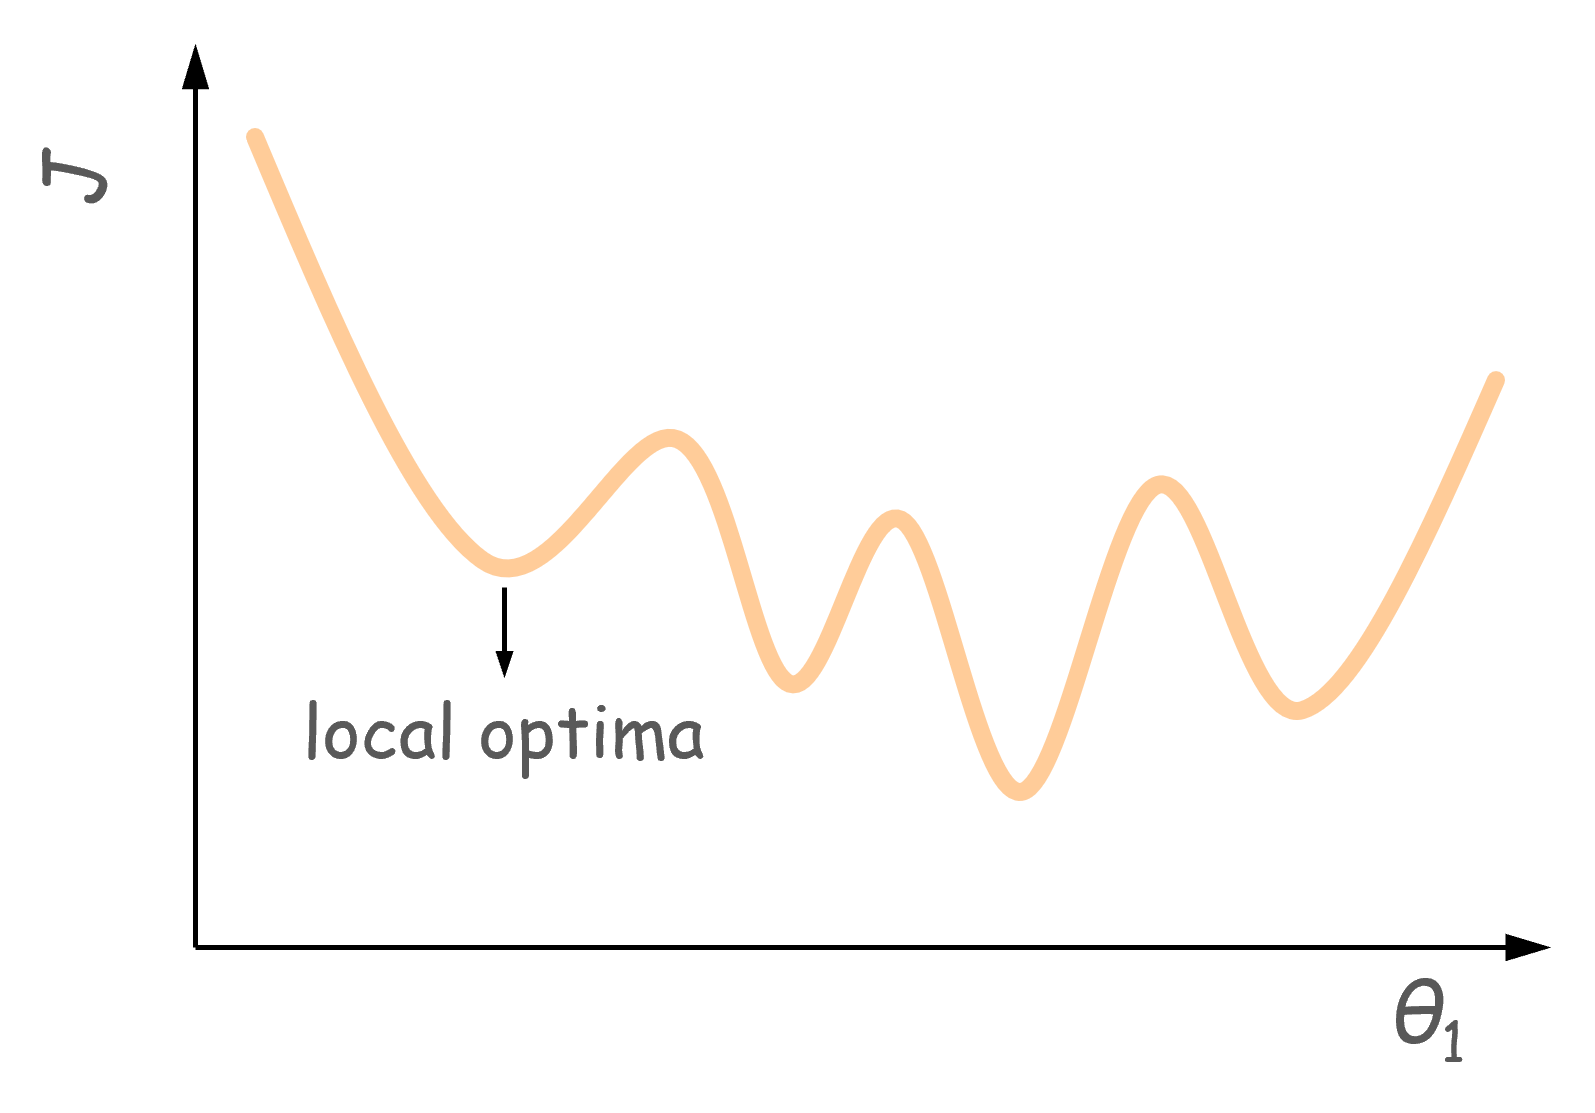
\includegraphics[width=1.8in]{./images/local_optima.png}
        \caption{Local optima}
    \end{figure}
\end{itemize}


\section{Model Representation}
\begin{itemize} 
    \item Assume there are $m$ sets of data and each data has $n$ features, then the raw input could be expressed as a $m \times n$ matrix $\mathbf{X}$:
    \begin{equation}
        \mathbf{X} =
        \left(
        \begin{matrix}
            x_1^{(1)} & x_2^{(1)} & \dots  & x_n^{(1)}\\
            x_1^{(2)} & x_2^{(2)} & \dots  & x_n^{(2)}\\
            \vdots    & \vdots    & \ddots & \vdots   \\
            x_1^{(m)} & x_2^{(m)} & \dots  & x_n^{(m)}\\
        \end{matrix}
        \right)_{m \times n}
    \end{equation}
    
    For polynomial functions, additional features can be created based on $x_1$,
    \begin{equation}
        h\left(x\right) = \theta_0 + \theta_1 x_1 + \theta_2 x_1^2 + \theta_3 x_1^3
    \end{equation}
    Then, the new features could be assumed as $x_2 = x_1^2$, $x_3 = x_1^3$
    
    \item In this course, $\mathbf{X}$ is usually expanded as a $m \times (n+1)$ matrix:
    \begin{equation}
        \mathbf{X} = 
        \left(
        \begin{matrix}
            x_0^{(1)} & x_1^{(1)} & \dots  & x_n^{(1)}\\
            x_0^{(2)} & x_1^{(2)} & \dots  & x_n^{(2)}\\
            \vdots    & \vdots    & \ddots & \vdots   \\
            x_0^{(m)} & x_1^{(m)} & \dots  & x_n^{(m)}\\
        \end{matrix}
        \right)_{m \times (n+1)}
    \end{equation}

    Normally, let $x_0^{(i)} = 1$ so that the first item of the hypothesis would be the constant $\theta_0$ (also called \textbf{bias}). The row component $\mathbf{x}^{(i)}$ of $\mathbf{X}$ means the $i^{th}$ set of training examples
    \footnote{In this document, a component is shown in a normal font such as $x^{(i)}_j$, a vector is shown in a bold font with a lowercase letter such as $\mathbf{x}^{(i)}$, a matrix is shown in a bold font with an uppercase letter such as $\mathbf{X}$.}:
    \begin{equation}
        \mathbf{x}^{(i)} = \left(\begin{matrix} x_0^{(i)} & x_1^{(i)} & \dots & x_n^{(i)} \end{matrix}\right)
    \end{equation}
    
    The columm component $\mathbf{x}_j$ of $\mathbf{X}$ means the $j^{th}$ feature of training examples:
    \begin{equation}
        \mathbf{x}_j = \left(\begin{matrix} x_j^{(1)} \\ x_j^{(2)} \\ \vdots \\ x_j^{(n)} \end{matrix}\right)
    \end{equation}

    \item The multivariable hypothesis function:
    \begin{equation}
        \begin{split}
            h^{(i)} & = \theta_0 x_0^{(i)} + \theta_1 x_1^{(i)} + \theta_2 x_2^{(i)} + \cdots + \theta_n x_n^{(i)}\\
            & = \left[ \begin{matrix} x_0^{(i)} & x_1^{(i)} & x_2^{(i)} & \dots & x_n^{(i)} \end{matrix} \right] 
                \left[ \begin{matrix} \theta_0 \\ \theta_1 \\ \theta_2 \\ \vdots \\ \theta_n \end{matrix} \right] \\
            & = \mathbf{x}^{(i)}\theta
        \end{split}
    \end{equation}                
    
    The relation between the hypothesis $h^{(i)}$ (seemed as \textbf{output}), the \textbf{input} $x_j^{(i)}$ and the \textbf{target} $y^{(i)}$ is:
    \begin{equation}
        \left(
            \begin{matrix}
                h^{(1)} \\
                h^{(2)} \\
                \vdots  \\
                h^{(m)} \\
            \end{matrix}
        \right) =
        \left(
        \begin{matrix}
            1         & x_1^{(1)} & \dots  & x_n^{(1)}\\
            1         & x_1^{(2)} & \dots  & x_n^{(2)}\\
            \vdots    & \vdots    & \ddots & \vdots   \\
            1         & x_1^{(m)} & \dots  & x_n^{(m)}\\
        \end{matrix}
        \right)
        \left(
        \begin{matrix}
            \theta_0\\
            \theta_1\\
            \vdots  \\
            \theta_n\\
        \end{matrix}
        \right)\rightarrow
        \left(
        \begin{matrix}
            y^{(1)} \\
            y^{(2)} \\
            \vdots  \\
            y^{(m)} \\
        \end{matrix}
        \right)
    \end{equation}
\end{itemize}


\section{Cost Function}
\begin{itemize}
    \item Define the cost function and derive a vectorized implementation
    \begin{equation}
        \begin{split}
            J\left(\theta\right)& = \frac{1}{2m}\sum_{i=1}^{m}\left( h^{(i)} - y^{(i)} \right)^2\\
            & = \frac{1}{2m}\sum_{i=1}^{m}\left( \theta_0x_0^{(i)} + \theta_1x_1^{(i)} + \dots + \theta_nx_n^{(i)} - y^{(i)} \right)^2\\
            & = \frac{1}{2m}\sum_{i=1}^{m}\left( \sum_{j=1}^{n}{\theta_j x_j^{(i)}} - y^{(i)} \right)^2\\
            & = \frac{1}{2m}\sum_{i=1}^{m}\left( \mathbf{x}^{(i)}\theta - y^{(i)} \right)^2\\
            & \textcolor{blue}{= \frac{1}{2m}\left( \mathbf{X}\theta - \mathbf{y} \right)\cdot\left( \mathbf{X}\theta - \mathbf{y} \right)}
        \end{split}
    \end{equation}
\end{itemize}
    

\section{Gradient Descent}
\begin{itemize} 

    \item Repeat until convergence
    \begin{equation}
        \begin{split}
            \theta_j& \coloneqq \theta_j - \alpha \frac{\partial}{\partial\theta_j}J\left(\theta\right)\\
                    & \coloneqq \theta_j - \frac{\alpha}{2m} \frac{\partial}{\partial\theta_j} \sum_{i=1}^{m}\left( h^{(i)} - y^{(i)} \right)^2\\
                    & \coloneqq \theta_j - \frac{\alpha}{m} \sum_{i=1}^{m}\left( h^{(i)} - y^{(i)} \right)\left(x_j^{(i)}\right)\\
        \end{split}
    \end{equation}
    for $j=0,1,\dots,n$

    \item In vectorized implementation
    \begin{equation}
        \begin{split}
            \theta & \coloneqq \theta - \frac{\alpha}{m}\mathbf{X}^T\left(\mathbf{X}\theta-\mathbf{y}\right)\\
        \end{split}
    \end{equation}

    \begin{proof}
        Let 
        \begin{equation}
            \nabla_j = \frac{1}{m}\sum_{i=1}^{m}(h^{(i)}-y^{(i)})x_j^{(i)}
        \end{equation}
        
        which is equivalent to
        \begin{equation}
            \nabla_j = \frac{1}{m}(\mathbf{h}-\mathbf{y})^T\mathbf{x}_j
        \end{equation}

        so
        \begin{equation}
            \begin{split}
                \left[ \begin{matrix} \nabla_0 & \nabla_1 & \dots & \nabla_n \end{matrix} \right] &= \frac{1}{m}(\mathbf{h}-\mathbf{y})^T \left[ \begin{matrix} \mathbf{x}_0 & \mathbf{x}_1 & \dots & \mathbf{x}_n \end{matrix} \right]\\
                                                                                                    &= \frac{1}{m}(\mathbf{h}-\mathbf{y})^T \mathbf{X} \\
            \end{split}
        \end{equation}

        thus
        \begin{equation}
            \left[\begin{matrix} \nabla_0 \\ \nabla_1 \\ \vdots \\ \nabla_n \end{matrix}\right] = \left( \frac{1}{m}(\mathbf{h}-\mathbf{y})^T \mathbf{X} \right)^T
                                                                                                = \frac{1}{m} \mathbf{X}^T (\mathbf{h}-\mathbf{y})
        \end{equation}
    \end{proof}

\end{itemize}


\section{Scaling and Normalization}
\begin{itemize} 
    \item We can speed up gradient descent by having each of our input values in roughly the same range. Ideally:
    \begin{equation}
        -1 \leq x^{(i)}_j \leq 1
    \end{equation}
    \item Two techniques to help with this are \textbf{feature scaling} and \textbf{mean normalization}.
    \item \textbf{Feature scaling} involves \textcolor{blue}{dividing} the input values by the range of the input variable, resulting in a new range of just 1.
    \item \textbf{Mean normalization} involves \textcolor{blue}{subtracting} the average value for that input variable resulting in a new average value of just zero. 
    \item To implement both of these techniques, adjust input values as shown in this formula:
    \begin{equation}
        x^{(i)}_j \coloneqq \frac{x^{(i)}_j-\mu^{(i)}}{s^{(i)}}
    \end{equation}
    where $\mu^{(i)}$ is the average of all the values for feature $i$ and $s^{(i)}$ is the range of values, or $s^{(i)}$ is the standard deviation.
\end{itemize}


\section{Normal Equation Method}
\begin{itemize}
    \item This method minimize $J$ by \textbf{explicitly} taking its derivatives with respect to the $\theta_j$, and setting them to zero. The normal equation formula is given below
    \begin{equation}\label{eqn:normal}
        \theta = \left(\mathbf{X}^T\mathbf{X}\right)^{-1}\mathbf{X}^T\mathbf{y}
    \end{equation}
    
    \item If $\left(\mathbf{X}^T\mathbf{X}\right)^{-1}$ is not invertible, the common causes might be having \textbf{redundant features} (i.e. there are linearly dependent features), or \textbf{too many features}  (e.g. $m \leq n$).
    Using \textbf{pinv} function rather than \textbf{inv} when implenting in Octave in this case.
    
    \item
    \begin{proof}
        The derivation of equation \ref{eqn:normal} is presented at \href{https://reurl.cc/0OY4zo}{Eli Bendersky's website}:
        \begin{equation}
            \begin{split}
                J(\theta) &= \frac{1}{2m} \left(\mathbf{X}\theta-\mathbf{y}\right)^{T} \left(\mathbf{X}\theta-\mathbf{y}\right)\\
                                   &= \frac{1}{2m} \left(\theta^{T}\mathbf{X}^{T} - \mathbf{y}^{T}\right) \left(\mathbf{X}\theta-\mathbf{y}\right)\\
                                   &= \frac{1}{2m} \left(\theta^{T}\mathbf{X}^{T}\mathbf{X}\theta - \theta^{T}\mathbf{X}^{T}\mathbf{y} - \mathbf{y}^{T}\mathbf{X}\theta + \mathbf{y}^{T}\mathbf{y}\right)\\
                                   &= \frac{1}{2m} \left(\theta^{T}\mathbf{X}^{T}\mathbf{X}\theta - 2\left(\mathbf{X}\theta\right)^{T}\mathbf{y} + \mathbf{y}^{T}\mathbf{y}\right)
            \end{split}
        \end{equation}
        
        Derive by $\theta$ and compare to 0, $\frac{\partial J}{\partial\theta} = 0$
        \begin{equation}
            \begin{split}
                2\mathbf{X}^T\mathbf{X}\theta - 2\mathbf{X}^T\mathbf{y} = 0\\
                2\mathbf{X}^T\mathbf{X}\theta = 2\mathbf{X}^T\mathbf{y}\\
                \theta = \left(\mathbf{X}^T\mathbf{X}\right)^{-1}\mathbf{X}^T\mathbf{y}
            \end{split}
        \end{equation}
    \end{proof}

    \item The following is a comparison of the algorithmic efficiency between \emph{gradient descent} and \emph{normal equation}
    \begin{table}[H]
        \renewcommand\arraystretch{1.5}
        \caption{Comparison of the algorithmic efficiency}
        \centering
        \begin{tabular}[t]{lll}     
            \hline 
            Items      & Gradient Descent             & Normal Equation          \\ 
            \hline 
            Complexity & $O\left(kn^2\right)$         & $O\left(n^3\right)$      \\ 
            Situation  & Works well when $n$ is large & Slow if $n$ is very large\\
            \hline
        \end{tabular}
    \end{table}
\end{itemize} 
